\section{IF}
\label{sec:if}

\subsection{Overview}
\label{sec:if-overview}

A \hyperref[sec:ada4940-2]{differential amplifier} is used to amplify the output of the mixer before
quantization by the \hyperref[sec:ltc2292]{ADC}.

\subsection{ADA4940-2 IF Differential Amplifier}
\label{sec:ada4940-2}

\subsubsection{Description}
\label{sec:ada4940-2-description}

The ADA4940-2 supports a max differential voltage at its input pins of $\pm 1 \si{V}$. \fixme{How do
I know that the ADL5802 outputs a differential voltage in this range. There are voltage gain
numbers on the mixer datasheet. However, I'm also confused about the power input to the mixer.}

\subsubsection{Pinout}
\label{sec:ada4940-2-pinout}

\label{tab:ada4940-2-pinout}
\begin{tabularx}{\textwidth}{l l X}
        \caption{The ADA4940-2 ADC pinout.}                                         \\
        \toprule
        \#    & Pin                   & Description                                 \\
        \midrule
        1     & -IN1                  &                                             \\
        2     & +FB1                  &                                             \\
        3, 4  & +V\textsubscript{S1}  & Positive supply voltage for the first differential amplifier. This is tied to
        +3.3V.                                                                      \\
        5     & -FB2                  &                                             \\
        6     & +IN2                  &                                             \\
        7     & -IN2                  &                                             \\
        8     & +FB2                  &                                             \\
        9, 10 & +V\textsubscript{S2}  & Positive supply voltage for the second differential amplifier. Also tied to
        +3.3V.                                                                      \\
        11    & V\textsubscript{OCM2} & Common-mode voltage of the second differential
        amplifier. This is set to 1.5V by the \hyperref[sec:ltc2292]{ADC}.          \\
        12    & +OUT2                 & Amplifier 2's positive differential output. \\
        13    & -OUT2                 & Amplifier 2's negative differential output. \\
        \bottomrule
\end{tabularx}

\subsubsection{Component Selection}
\label{sec:ada4940-2-component-selection}

The components between \hyperref[sec:adl5802]{ADL5802} and the IF amplifier form a high-pass filter
with a transfer function shown in Fig.~\ref{fig:mixer-if-amp-filter}. The filter has a flat gain of
$-10 \si{dBV}$ from about $30 \si{kHz}$ through several hundred $\si{kHz}$ and still stays below
$-5 \si{dBV}$ up to $1 \si{MHz}$. The phase angle is also mostly flat at 0 in this region. The
transfer function was performed using Ngspice with KiCad, and the schematic for it is shown in
Fig.~\ref{fig:mixer-if-amp-filter-schematic}.

\begin{figure}[h]
        \centering
        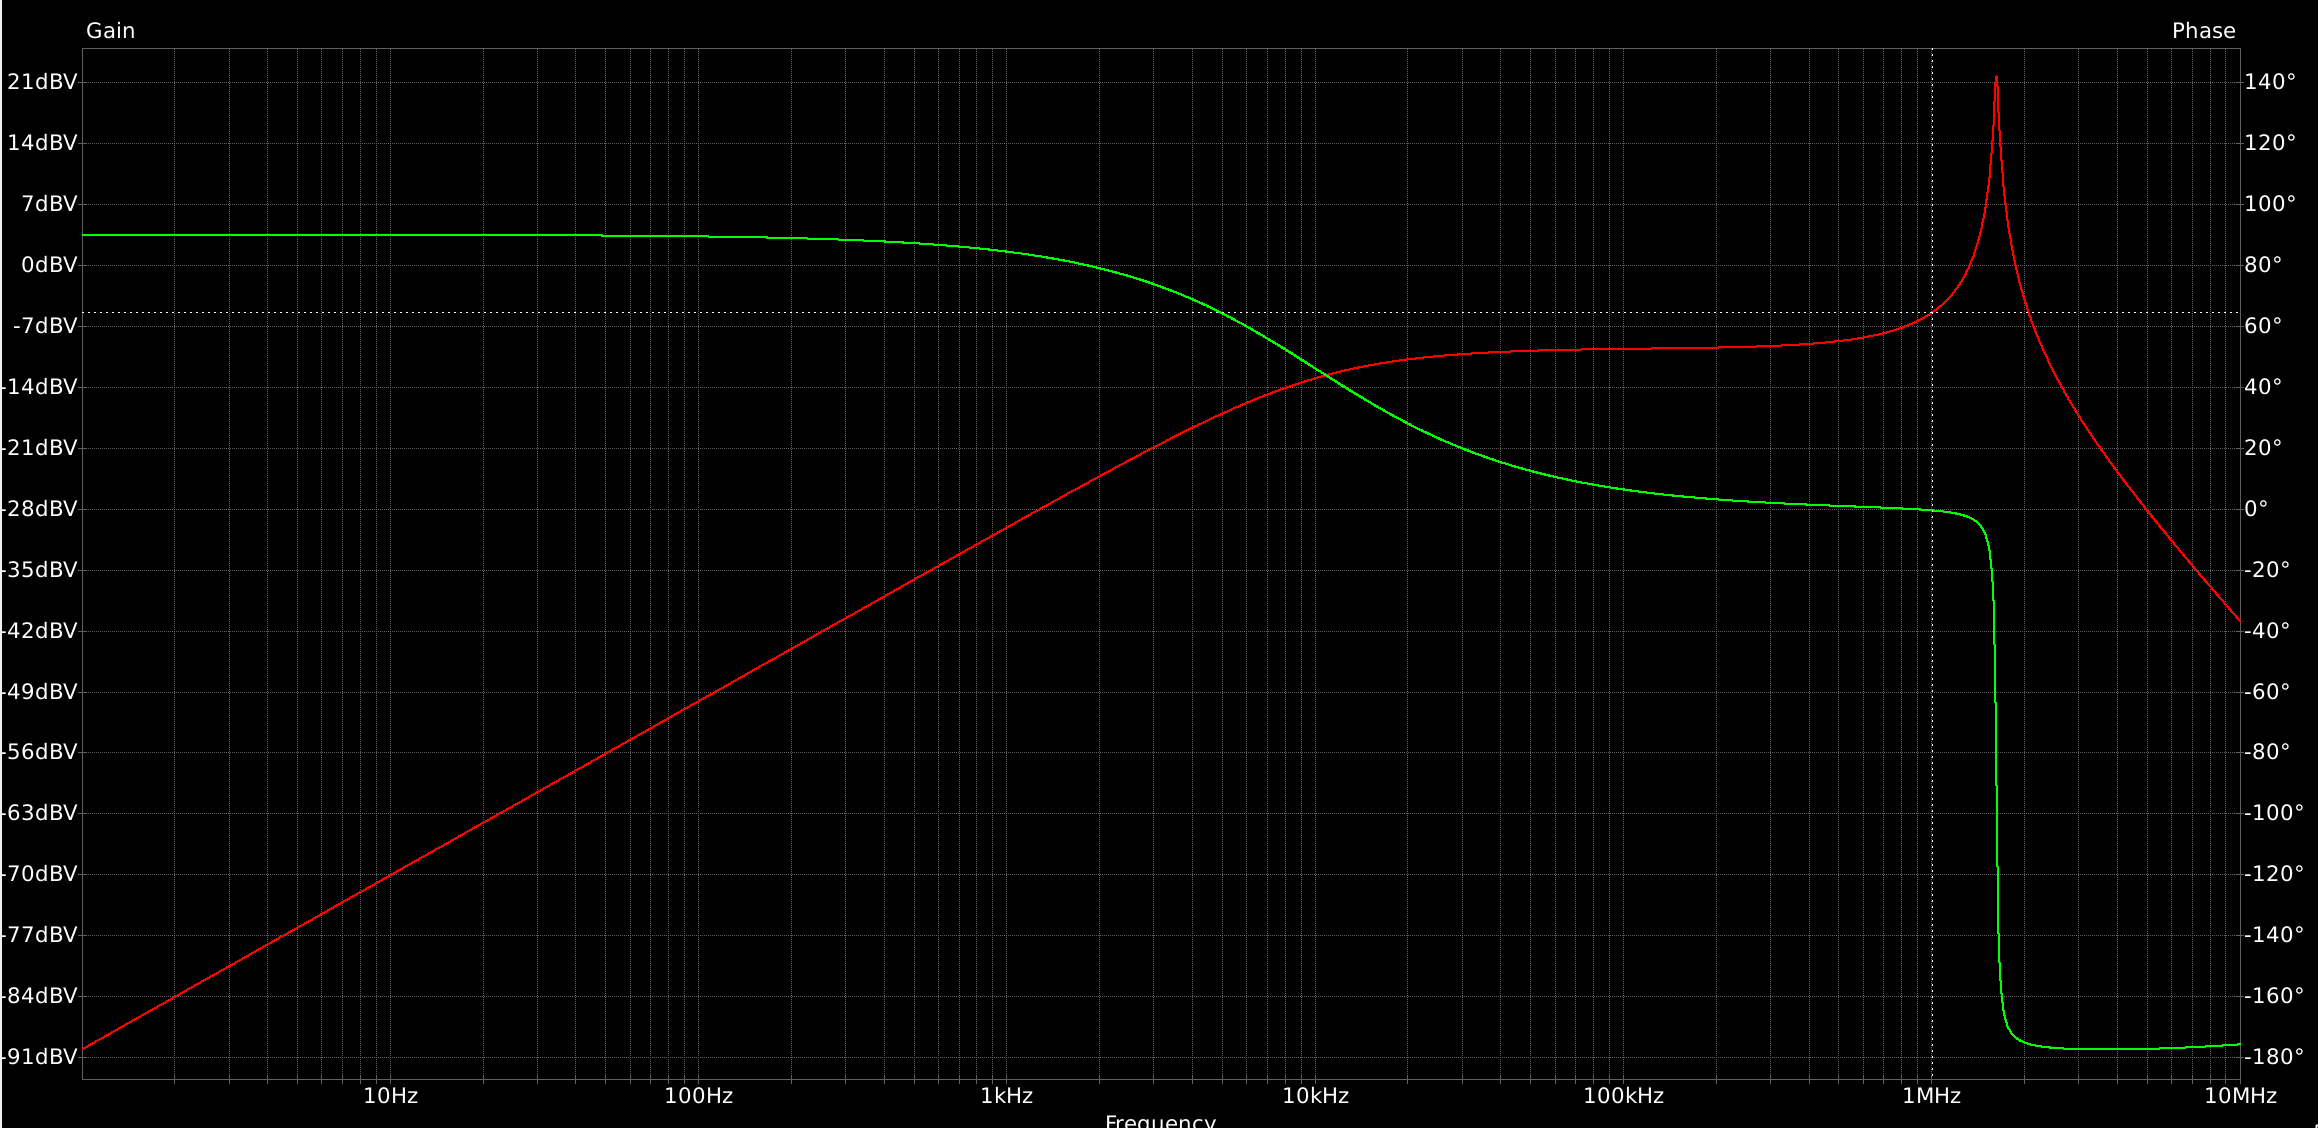
\includegraphics[width=\textwidth]{data/mixer-if-amp-filter}
        \caption{High-pass filter at the IF amplifier differential inputs.}
        \label{fig:mixer-if-amp-filter}
\end{figure}

\begin{figure}[h]
        \centering
        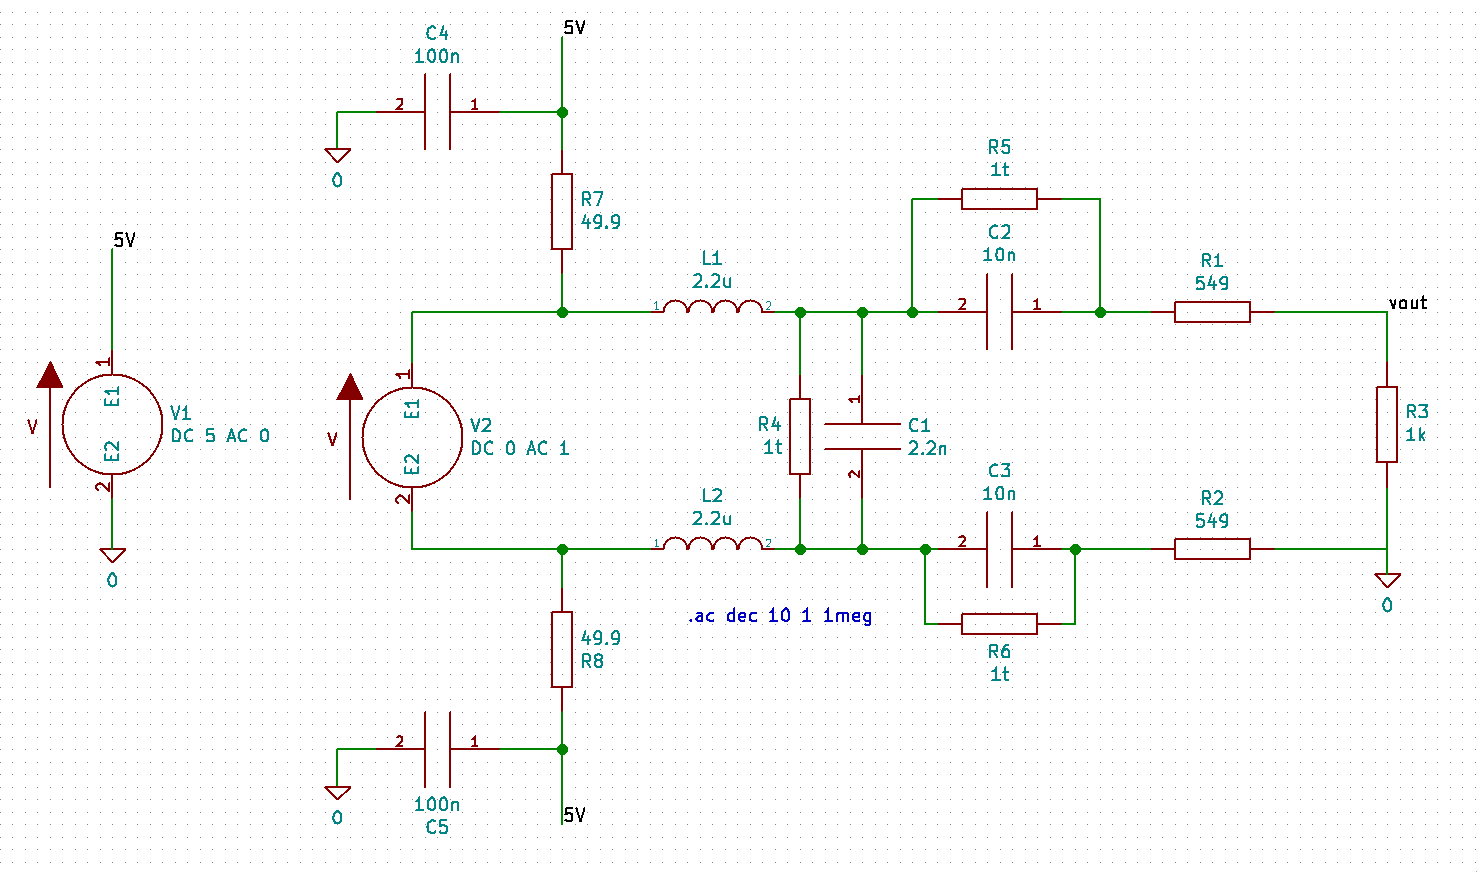
\includegraphics[width=\textwidth]{data/mixer-if-amp-filter-schematic}
        \caption{Schematic for the Ngspice simulation of the high-pass filter. The
          $1 \si{\protect\bm{T\Omega}}$ resistors in parallel with the capacitors provide a DC
          current path to ground and are necessary for the simulation to work.}
        \label{fig:mixer-if-amp-filter-schematic}
\end{figure}

\subsubsection{PCB Layout}
\label{sec:ada4940-2-pcb}

%%% Local Variables:
%%% mode: latex
%%% TeX-master: "fmcw-radar"
%%% End:
